\chapter{Mutual Information and the Data Processing Inequality}
\label{ch:mutual_information}

\section{The Currency of Representation}

If entropy is the measure of uncertainty, mutual information is the measure of insight. When a neural network processes an image to classify a breed of dog, we do not care about the entropy of the hidden layers in isolation. We care about how much those hidden layers actually know about the target label. Mutual information is the mathematical formalized answer to the question: ``How much does knowing $X$ reduce my uncertainty about $Y$?''

In deep learning, mutual information is arguably the most critical quantity. It serves as the primary currency exchanged during representation learning. Contrastive learning methods like SimCLR and InfoNCE are, at their core, algorithms designed to maximize the mutual information between different augmentations of the same image. The Information Bottleneck principle frames deep learning entirely as an optimization of mutual information: maximizing the mutual information between the representation and the label, while minimizing the mutual information between the representation and the raw input. 

Yet, there is a strict, physical constraint on this currency. Information cannot be spontaneously generated by processing data. A deterministic function applied to a signal can only destroy information or preserve it; it can never add new information about the original source. This profound truth is known as the Data Processing Inequality (DPI). The DPI governs the forward pass of every neural network. As data flows from the input layer through the hidden layers to the output, the mutual information with the target label monotonically decreases (or stays flat). The magic of deep learning is not in creating information, but in stripping away the irrelevant noise so that the remaining information is linearly separable.

\section{Mathematical Definitions}

Building upon the definitions of entropy and conditional entropy from previous chapters, we formally define mutual information.

\begin{definition}[Mutual Information]
The mutual information $I(X; Y)$ between two discrete random variables $X$ and $Y$ is the reduction in uncertainty of $X$ due to the knowledge of $Y$:
\begin{equation}
    I(X; Y) = H(X) - H(X|Y)
\end{equation}
\end{definition}

Because of the symmetry of joint entropy ($H(X,Y) = H(Y,X)$), we can rewrite this in several insightful ways:
\begin{align}
    I(X; Y) &= H(Y) - H(Y|X) \label{eq:mi_sym1} \\
    I(X; Y) &= H(X) + H(Y) - H(X, Y) \label{eq:mi_sym2} \\
    I(X; Y) &= \sum_{x \in \mathcal{X}} \sum_{y \in \mathcal{Y}} p(x, y) \log \frac{p(x, y)}{p(x)p(y)} \label{eq:mi_kl}
\end{align}

Equation~\ref{eq:mi_kl} reveals a deep connection: mutual information is the Kullback-Leibler (KL) divergence between the joint distribution $p(x,y)$ and the product of the marginal distributions $p(x)p(y)$. It measures how far the variables are from being strictly independent.

\begin{theorem}[Non-negativity of Mutual Information]
For any two random variables $X$ and $Y$, $I(X;Y) \geq 0$, with equality if and only if $X$ and $Y$ are independent.
\end{theorem}
\begin{proof}
By definition, $I(X;Y) = H(X) - H(X|Y)$. Since conditioning reduces entropy (Corollary from Chapter~\ref{ch:joint_conditional}), $H(X|Y) \leq H(X)$, implying $I(X;Y) \geq 0$. Equality holds if $H(X|Y) = H(X)$, meaning knowledge of $Y$ does not change the distribution of $X$, which is the definition of independence.
\end{proof}

\subsection{The Data Processing Inequality}

To discuss the flow of information through a neural network, we must define a Markov chain. Random variables $X$, $Y$, and $Z$ form a Markov chain $X \to Y \to Z$ if the conditional distribution of $Z$ depends only on $Y$ and is conditionally independent of $X$. Mathematically: $p(z|x,y) = p(z|y)$. 

In deep learning, the sequence of layers $X \to H_1 \to H_2 \to \dots \to \hat{Y}$ strictly forms a Markov chain.

\begin{theorem}[Data Processing Inequality]
\label{thm:dpi}
If $X \to Y \to Z$ forms a Markov chain, then the mutual information cannot increase:
\begin{equation}
    I(X; Y) \geq I(X; Z)
\end{equation}
\end{theorem}

\begin{proof}
By the chain rule for mutual information, we can expand $I(X; Y, Z)$ in two different ways:
\begin{align}
    I(X; Y, Z) &= I(X; Z) + I(X; Y | Z) \label{eq:dpi1} \\
    I(X; Y, Z) &= I(X; Y) + I(X; Z | Y) \label{eq:dpi2}
\end{align}
Since $X \to Y \to Z$ is a Markov chain, $X$ and $Z$ are conditionally independent given $Y$. Therefore, $I(X; Z | Y) = 0$.
Substituting this into Equation~\ref{eq:dpi2} gives $I(X; Y, Z) = I(X; Y)$.
Equating this with Equation~\ref{eq:dpi1}:
\begin{equation}
    I(X; Y) = I(X; Z) + I(X; Y | Z)
\end{equation}
Since mutual information is always non-negative, $I(X; Y | Z) \geq 0$, which requires that:
\begin{equation}
    I(X; Y) \geq I(X; Z)
\end{equation}
\end{proof}

\begin{figure}[ht]
    \centering
    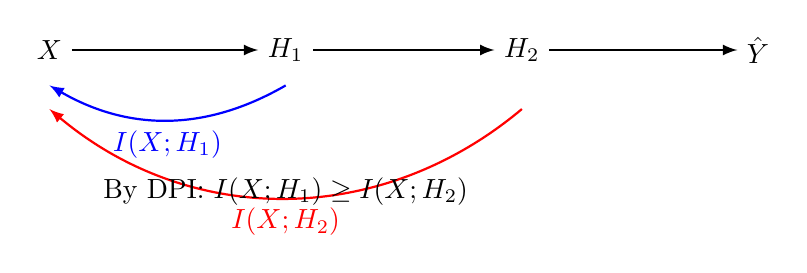
\begin{tikzpicture}[>=latex, scale=1.5]
        \node (x) at (0, 0) {$X$};
        \node (h1) at (2, 0) {$H_1$};
        \node (h2) at (4, 0) {$H_2$};
        \node (y) at (6, 0) {$\hat{Y}$};
        
        \draw[->, thick] (x) -- (h1);
        \draw[->, thick] (h1) -- (h2);
        \draw[->, thick] (h2) -- (y);
        
        \draw[<-, thick, blue, bend right=30] (0, -0.3) to node[below] {$I(X;H_1)$} (2, -0.3);
        \draw[<-, thick, red, bend right=40] (0, -0.5) to node[below] {$I(X;H_2)$} (4, -0.5);
        
        \node at (2, -1.2) {By DPI: $I(X;H_1) \geq I(X;H_2)$};
    \end{tikzpicture}
    \caption{Information flow through the layers of a neural network. Information about the input $X$ can only degrade as it moves deeper into the network.}
    \label{fig:dpi_network}
\end{figure}

The DPI (Figure~\ref{fig:dpi_network}) implies that no clever manipulation of $Y$ can uncover more information about $X$ than was originally present in $Y$. 

\subsection{Worked Numerical Example}

Suppose a binary input signal $X \in \{0,1\}$ is transmitted through two noisy channels in sequence to produce $Y$ and then $Z$. 
Let $p(x=0) = 0.5$ and $p(x=1) = 0.5$.
The first channel flips the bit with probability $p=0.1$. Thus, $p(y \neq x) = 0.1$.
The second channel flips the bit again with probability $q=0.2$. Thus, $p(z \neq y) = 0.2$.

First, let's find $I(X; Y)$. 
$H(X) = 1$ bit. 
The conditional entropy $H(X|Y)$ depends on the error rate of the channel. Since it's a symmetric binary channel with crossover probability 0.1, $H(X|Y) = H(0.1) = -0.1\log_2 0.1 - 0.9\log_2 0.9 \approx 0.469$ bits.
\begin{equation*}
    I(X; Y) = H(X) - H(X|Y) = 1 - 0.469 = 0.531 \text{ bits.}
\end{equation*}

Now, what is $I(X; Z)$? 
The total probability of a bit flip from $X$ to $Z$ happens if the first channel flips it and the second doesn't, OR the first doesn't and the second does.
$P(Z \neq X) = (0.1)(0.8) + (0.9)(0.2) = 0.08 + 0.18 = 0.26$.
So the effective channel from $X$ to $Z$ has an error rate of 0.26.
$H(X|Z) = H(0.26) = -0.26\log_2 0.26 - 0.74\log_2 0.74 \approx 0.827$ bits.
\begin{equation*}
    I(X; Z) = H(X) - H(X|Z) = 1 - 0.827 = 0.173 \text{ bits.}
\end{equation*}

As expected by the Data Processing Inequality, $I(X; Y) > I(X; Z)$ ($0.531 > 0.173$). Information is lost in transit.

\begin{figure}[ht]
    \centering
    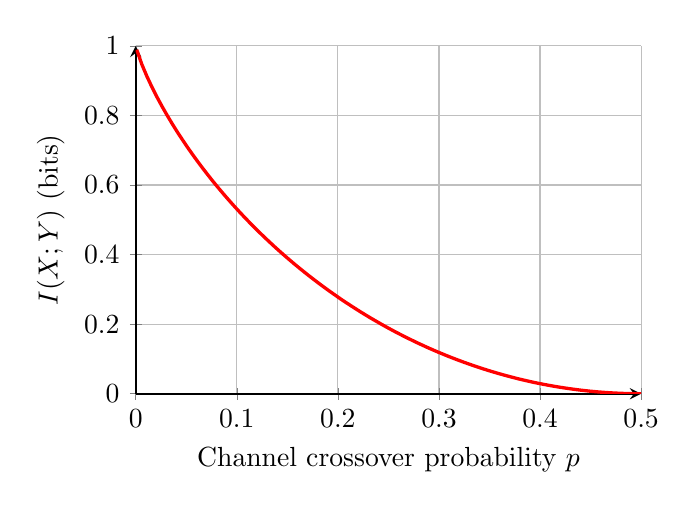
\begin{tikzpicture}[>=latex, scale=1]
        \begin{axis}[
            width=8cm, height=6cm,
            xlabel={Channel crossover probability $p$},
            ylabel={$I(X;Y)$ (bits)},
            xmin=0, xmax=0.5,
            ymin=0, ymax=1,
            grid=major,
            axis lines=left,
            thick
        ]
        \addplot[domain=0.001:0.5, samples=100, red, very thick] 
            {1 - (-x*log2(x) - (1-x)*log2(1-x))};
        \end{axis}
    \end{tikzpicture}
    \caption{Mutual information between input and output of a binary symmetric channel as a function of error rate $p$. As noise increases, mutual information drops to zero.}
    \label{fig:capacity}
\end{figure}

\begin{horizon}
The strict formulation of the Data Processing Inequality forms an ironclad bound on deep learning representations: a layer $H_n$ can never contain more information about the target label $Y$ than the previous layer $H_{n-1}$. This mathematically justifies why deep networks must focus on discarding irrelevant noise, rather than creating signal.

However, in practice, deep networks are not evaluated on raw mutual information, but on "usable" or "accessible" information. While $I(X;H_1) \geq I(X;H_n)$, the information in $H_1$ is highly entangled and non-linear, whereas the information in $H_n$ is linearly separable by a simple softmax layer. 

It is conjectured that deep learning operates by sacrificing total mutual information $I(X;Z)$ in exchange for maximizing the linearly decodable mutual information $I_{lin}(Y;Z)$. An open question is how to rigorously define this "usable" information metric. If we can bound the gap between $I(Y;Z)$ and $I_{lin}(Y;Z)$, we could theoretically predict a network's test accuracy purely by examining the geometry of its latent space, without running inference. Future work attempting to bridge classical Shannon information with Vapnik-Chervonenkis (VC) theory might yield a modified DPI that accounts for computational complexity.
\end{horizon}

\section*{Summary}
Mutual information $I(X;Y)$ measures the amount of information that one variable contains about another. It is symmetric, non-negative, and intimately related to KL divergence. Crucially, the Data Processing Inequality (DPI) establishes that post-processing cannot increase information. In a Markov chain $X \to Y \to Z$, $I(X;Y) \geq I(X;Z)$. This fundamental theorem reveals that neural networks do not synthesize new information about the target; rather, they transform existing information into a more accessible format while deliberately discarding irrelevant nuisance variables.

\section*{Exercises}
\begin{enumerate}
    \item \textbf{Venn Diagram Proofs:} Using the definitions of $H(X)$, $H(X,Y)$, and $H(X|Y)$, prove that $I(X;Y) = H(X) + H(Y) - H(X,Y)$.
    \item \textbf{Deterministic Bottleneck:} Consider an image classifier where $x \in \mathbb{R}^{784}$ (MNIST) is mapped to a bottleneck $z \in \mathbb{R}^{2}$, and then to a prediction $\hat{y}$. Why must the classification accuracy be bounded by the mutual information capacity of the 2D bottleneck? 
    \item \textbf{Sufficient Statistics:} A statistic $T(X)$ is called a sufficient statistic for a parameter $\theta$ if $I(\theta; X) = I(\theta; T(X))$. Show that if $T(X)$ is sufficient, the DPI holds with equality in the chain $\theta \to X \to T(X)$. 
    \item \textbf{Mutual Information of Continuous Variables:} Why does $I(X;Y)$ remain perfectly well-defined and positive for continuous variables, even though differential entropy $h(X)$ can be negative?
\end{enumerate}

% TODO-CITE: Ensure all named results are cited.
